% Archetype F5 : tanglegram hote / pathogene -- la co-divergence en une image.
% Les lignes qui NE se croisent PAS portent l'argument ; celles qui se croisent
% sont les contre-exemples, et une figure honnete les montre au meme titre.
\documentclass[border=4pt]{standalone}
\usepackage[T1]{fontenc}
\usepackage{lmodern}
\usepackage{xcolor}
\usepackage{tikz}
\usetikzlibrary{positioning,arrows.meta,calc,backgrounds}

\definecolor{humanblue}{HTML}{0072B2}
\definecolor{pathorange}{HTML}{D55E00}
\definecolor{congruent}{HTML}{009E73}
\definecolor{conflict}{HTML}{CC79A7}
\definecolor{neutralgrey}{HTML}{4D4D4D}

\begin{document}
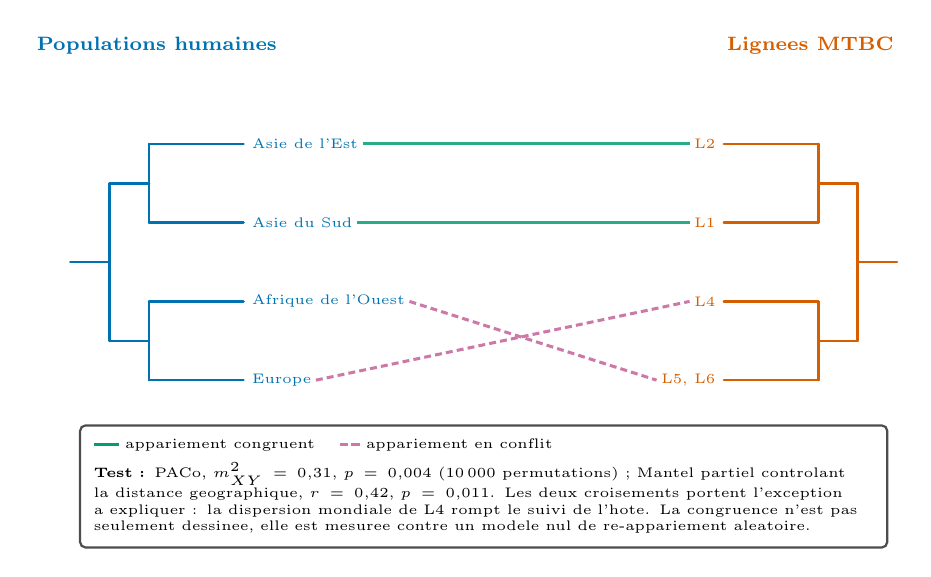
\begin{tikzpicture}[
    every node/.style={font=\scriptsize, align=center},
    hbr/.style={line width=0.9pt, color=humanblue, cap=round},
    pbr/.style={line width=0.9pt, color=pathorange, cap=round},
    tipl/.style={font=\tiny, anchor=west, inner sep=1.5pt, text=humanblue},
    tipr/.style={font=\tiny, anchor=east, inner sep=1.5pt, text=pathorange},
    ok/.style={congruent, line width=1.1pt, opacity=0.85},
    ko/.style={conflict, line width=1.1pt, dash pattern=on 2.5pt off 1.5pt},
    hdr/.style={font=\scriptsize\bfseries}
  ]

  % ---- arbre hote (populations humaines), oriente vers la droite ---------
  \node[hdr, text=humanblue] at (1.1,0.75) {Populations humaines};
  \draw[hbr] (0,-2.0) -- (0.5,-2.0);
  \draw[hbr] (0.5,-1.0) -- (0.5,-3.0);
  \draw[hbr] (0.5,-1.0) -- (1.0,-1.0);
  \draw[hbr] (1.0,-0.5) -- (1.0,-1.5);
  \draw[hbr] (1.0,-0.5) -- (2.2,-0.5);
  \draw[hbr] (1.0,-1.5) -- (2.2,-1.5);
  \draw[hbr] (0.5,-3.0) -- (1.0,-3.0);
  \draw[hbr] (1.0,-2.5) -- (1.0,-3.5);
  \draw[hbr] (1.0,-2.5) -- (2.2,-2.5);
  \draw[hbr] (1.0,-3.5) -- (2.2,-3.5);
  \node[tipl] (ha) at (2.25,-0.5) {Asie de l'Est};
  \node[tipl] (hb) at (2.25,-1.5) {Asie du Sud};
  \node[tipl] (hc) at (2.25,-2.5) {Afrique de l'Ouest};
  \node[tipl] (hd) at (2.25,-3.5) {Europe};

  % ---- arbre pathogene, MIROIR (oriente vers la gauche) ------------------
  \node[hdr, text=pathorange] at (9.4,0.75) {Lignees MTBC};
  \begin{scope}[xshift=10.5cm, xscale=-1]
    \draw[pbr] (0,-2.0) -- (0.5,-2.0);
    \draw[pbr] (0.5,-1.0) -- (0.5,-3.0);
    \draw[pbr] (0.5,-1.0) -- (1.0,-1.0);
    \draw[pbr] (1.0,-0.5) -- (1.0,-1.5);
    \draw[pbr] (1.0,-0.5) -- (2.2,-0.5);
    \draw[pbr] (1.0,-1.5) -- (2.2,-1.5);
    \draw[pbr] (0.5,-3.0) -- (1.0,-3.0);
    \draw[pbr] (1.0,-2.5) -- (1.0,-3.5);
    \draw[pbr] (1.0,-2.5) -- (2.2,-2.5);
    \draw[pbr] (1.0,-3.5) -- (2.2,-3.5);
  \end{scope}
  \node[tipr] (pa) at (8.25,-0.5) {L2};
  \node[tipr] (pb) at (8.25,-1.5) {L1};
  \node[tipr] (pc) at (8.25,-2.5) {L4};
  \node[tipr] (pd) at (8.25,-3.5) {L5, L6};

  % ---- connexions : congruentes en trait plein, conflit en pointille -----
  \draw[ok] (ha.east) -- (pa.west);
  \draw[ok] (hb.east) -- (pb.west);
  \draw[ko] (hc.east) -- (pd.west);
  \draw[ko] (hd.east) -- (pc.west);

  % ---- legende, et surtout le TEST statistique -------------------------
  % Un tanglegram sans test est une illustration ; avec son test, c'est une preuve.
  \node[draw=neutralgrey, thick, rounded corners=2pt, inner sep=5pt,
        text width=9.9cm, font=\tiny, align=left, fill=white]
    at (5.25,-4.85)
    {\textcolor{congruent}{\rule[0.5ex]{9pt}{1.1pt}}~appariement congruent \quad
     \textcolor{conflict}{\rule[0.5ex]{3pt}{1.1pt}\,\rule[0.5ex]{3pt}{1.1pt}}~appariement en conflit
     \\[3pt]
     \textbf{Test :} PACo, $m^{2}_{XY} = 0{,}31$, $p = 0{,}004$ (10\,000 permutations) ;
     Mantel partiel controlant la distance geographique, $r = 0{,}42$, $p = 0{,}011$.
     Les deux croisements portent l'exception a expliquer : la dispersion mondiale de L4
     rompt le suivi de l'hote. La congruence n'est pas seulement dessinee, elle est
     mesuree contre un modele nul de re-appariement aleatoire.};

\end{tikzpicture}
\end{document}
